% context: 9th-grade physics pretest (homework), Unit 2 kinematics with Unit 1 review;
%        practice for the unit test on 19 November 2026. Fairly easy by design: it is
%        a skills check, one or two items per skill. No early-finisher section
% topic: significant figures, rounding, scientific notation with a calculator; mental
%        math aimed at the 2-6DN errors (metric direction, squaring a decimal, km/h to
%        m/s, decimal minutes, d = vt with minutes); a one-chain unit conversion; a
%        rate problem in two steps; distance vs displacement, average speed vs
%        velocity; braking; a ball thrown up; reading a velocity-time graph
% structure: four pages, two problems per page, generous room to work
% skills (for competency scoring): Q1 sig figs, rounding, sci notation, calculator;
%        Q2 mental math; Q3 unit conversion; Q4 rate problem; Q5 displacement and
%        average velocity; Q6 constant-acceleration equations; Q7 free fall;
%        Q8 motion graphs
% data: Moon distance 384 400 km and c = 3.00 x 10^8 m/s (contexts.md #10); Taipei 101
%        elevator 1010 m/min (contexts.md #3); New York walking speed 1.4 m/s and
%        20 blocks to the mile (contexts.md #5); UK Highway Code 50 mi/h braking
%        distance 38 m, with a = -6.4 m/s^2 from 2-3HW. The walk, the throw and the
%        car's graph are chosen values
\documentclass[12pt, twoside]{article}
%\documentclass[12pt, twoside]{article}
\usepackage[letterpaper, margin=1in, headsep=0.2in]{geometry}
\setlength{\headheight}{0.6in}
%\usepackage[english]{babel}
\usepackage[utf8]{inputenc}
\usepackage{microtype}
\usepackage{amsmath}
\usepackage{amssymb}
%\usepackage{amsfonts}
\usepackage[nomessages]{fp} %\FPeval{\var-name}{2*sin(pi/6)}
\usepackage{siunitx} %units in math. eg 20\milli\meter
\usepackage{yhmath} % for arcs, overparenth command
\usepackage{tikz} %graphics
\usetikzlibrary{quotes, angles, arrows, arrows.meta}
\usepackage{graphicx} %consider setting \graphicspath{{images/}}
\usepackage{parskip} %no paragraph indent
\usepackage{enumitem}
\usepackage{multicol}
\usepackage{venndiagram}

\usepackage{fancyhdr}
\pagestyle{fancy}
\fancyhf{}
\renewcommand{\headrulewidth}{0pt} % disable the underline of the header
\raggedbottom
\hfuzz=2mm %suppresses overfull box warnings

\usepackage{hyperref}
\usepackage{float}

\title{Physics}
\author{Chris Huson}
\date{November 2026}

\fancyhead[LE]{\thepage}
\fancyhead[RO]{\thepage \\ Nickname: \hspace{2.25cm} \,\\ \,}
\fancyhead[LO]{La Scuola d'Italia / Huson / Physics \\* 12 November 2026}

\newcommand{\blank}[1][2.4cm]{\rule{#1}{0.4pt}}

\begin{document}

\subsubsection*{2.8 PreTest: Kinematics (homework)}

\textbf{Reference (provided).} \quad
average speed $= \dfrac{\text{distance}}{\text{time}}$ \quad
$\bar{v} = \dfrac{\text{displacement}}{\text{time}}$ \quad
$a = \dfrac{v - v_0}{t}$

\vspace{0.1cm}
When the acceleration $a$ is constant:

{\hspace{0.5cm}%
\renewcommand{\arraystretch}{1.8}%
\begin{tabular}{l @{\hspace{2cm}} l}
  $v = v_0 + at$ & $v^2 = v_0^2 + 2a(x - x_0)$ \\
  $x = x_0 + v_0 t + \frac{1}{2}at^2$ & $\bar{v} = \dfrac{v + v_0}{2}$
\end{tabular}}

\vspace{0.1cm}
For a falling object, write $y$ in place of $x$, and $a = g = 9.80$ m/s$^2$ downward.

1 min = 60 s \quad 1 h = 3600 s \quad 1 km = 1000 m \quad 1 m/s = 3.6 km/h \quad
1 mile = 1609 m

\vspace{0.1cm}
Show your work, with units, in the space below each question.

\vspace{0.2cm}

\begin{enumerate}[itemsep=0.6cm]

\item Measurement review. Use a calculator.
  \begin{enumerate}[itemsep=0.6cm]
    \item How many significant figures are in \num{0.00470} kg? \hfill \blank
    \item Round 9.80665 m/s$^2$ to three significant figures. \hfill \blank
    \item The Moon is \num{384400} km from Earth. Write this distance in meters, in
      scientific notation. \hfill \blank
    \item Light travels at $3.00 \times 10^{8}$ m/s. How long does light from the
      Moon take to reach Earth?
      \vspace{3.0cm}
  \end{enumerate}

\item Mental math. No calculator: write just the answer, with its units.
  \begin{multicols}{2}
    \begin{enumerate}[itemsep=0.6cm, series=mm]
      \item 0.4 m = \blank\ mm
      \item $0.3^2 = $ \blank
      \item 54 km/h = \blank\ m/s
      \item 90 s = \blank\ min
      \item 20 min = \blank\ h (fraction)
      \item[]
    \end{enumerate}
  \end{multicols}
  \begin{enumerate}[resume=mm, itemsep=0.6cm]
    \item A car drives at 60 km/h for 30 min. How far does it go? \hfill \blank
  \end{enumerate}

\newpage

\item The elevators in Taipei 101, once the fastest in the world, are rated at
  1010 m/min. Write each conversion as one chain of unit factors.
  \begin{enumerate}[itemsep=0.4cm]
    \item Convert 1010 m/min to m/s.
      \vspace{4.5cm}
    \item Convert 1010 m/min to km/h.
      \vspace{4.5cm}
  \end{enumerate}

\item New Yorkers walk at about 1.4 m/s. Twenty north--south blocks in Manhattan make
  one mile, 1609 m. How many minutes does it take to walk the 20 blocks?

  Step 1: find the time in seconds. \quad Step 2: convert it to minutes.

\newpage

\item Take the school entrance as the origin, with east positive. A student walks
  12 m east in 8.0 s, then 20 m west in 12.0 s. Draw each displacement as an arrow
  above the number line.

  \begin{center}
  \begin{tikzpicture}[scale=0.55]
    \draw[<->, thick] (-11,0) -- (15,0) node[right]{$x$ (m)};
    \foreach \x in {-10,...,14} \draw (\x,0.12) -- (\x,-0.12);
    \foreach \x in {-10,-8,...,14} \node[below] at (\x,-0.12) {\small \x};
    \node[above] at (0,0.1) {\scriptsize entrance};
    \path (0,0) -- (0,1.8); % room above the line for the arrows
    % Solution arrows — uncomment to see the answer
    %\draw[->, very thick] (0,0.8) -- (12,0.8) node[midway, above]{\small $+12$ m};
    %\draw[->, very thick] (12,1.6) -- (-8,1.6) node[midway, above]{\small $-20$ m};
  \end{tikzpicture}
  \end{center}

  \begin{enumerate}[itemsep=0.6cm]
    \item Where does the student end up? \hfill $x = $ \blank
    \item Distance walked = \blank \hfill Displacement = \blank
    \item Find the average speed and the average velocity for the whole walk.
      \vspace{3.5cm}
  \end{enumerate}

\item A car is driving at 50 mi/h (22.4 m/s) when the driver brakes hard. In 2.3 you
  found that the car slows down at $a = -6.4$ m/s$^2$.
  \begin{enumerate}[itemsep=0.4cm]
    \item How long does the car take to stop?
      \vspace{3.5cm}
    \item Find the braking distance. The UK Highway Code gives 38 m at 50 mi/h. Does
      your answer agree?
  \end{enumerate}

\newpage

\item A ball is thrown straight up at 19.6 m/s. Take \emph{up} as positive.
  \begin{enumerate}[itemsep=0.4cm]
    \item At the highest point, what is the ball's velocity? What is its
      acceleration?
      \vspace{1.6cm}
    \item How long does the ball take to reach the highest point?
      \vspace{2.8cm}
    \item How high does it go?
      \vspace{2.8cm}
  \end{enumerate}

\item The graph shows the velocity of a car pulling away from a traffic light.

  \begin{minipage}[t]{0.58\linewidth}
    \vspace{0pt}
    \begin{tikzpicture}[x=0.82cm, y=0.32cm]
      \draw[gray!25, thin, xstep=0.5, ystep=1] (0,0) grid (8,14);
      \draw[gray!60, xstep=1, ystep=2] (0,0) grid (8,14);
      \draw[->, thick] (0,0) -- (8.5,0) node[right]{\small $t$ (s)};
      \draw[->, thick] (0,0) -- (0,15) node[above]{\small $v$ (m/s)};
      \foreach \t in {0,...,8} \node[below] at (\t,0) {\scriptsize \t};
      \foreach \v in {2,4,...,14} \node[left] at (0,\v) {\scriptsize \v};
      \draw[very thick] (0,0) -- (4,12) -- (8,12);
    \end{tikzpicture}
  \end{minipage}
  \hfill
  \begin{minipage}[t]{0.38\linewidth}
    \vspace{0pt}
    \begin{enumerate}[itemsep=1.6cm]
      \item What is the car's velocity at \mbox{$t = 2.0$ s}?
      \item Find the car's acceleration from 0 to 4.0 s. Give the units.
      \item What is the acceleration from 4.0~s to 8.0~s? What is the car doing?
    \end{enumerate}
  \end{minipage}

\end{enumerate}
\end{document}
